\scanpage{100}\mspage{91}
\figure{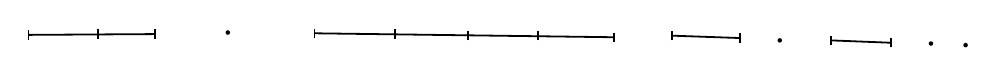
\begin{tikzpicture}[x=.1mm,y=.1mm,line width=.65pt]
\draw (0,1)--(161,2) (363,3)--(743,-2) (817,0)--(903,-3) (1019,-6)--(1095,-9);
\foreach \x/\y in {0/1,88/2,161/2,363/3,465/2,558/0,647/0,743/-2,817/0,903/-3,1019/-6,1095/-9}
 {\draw (\x,\y-6)--(\x,\y+6);}
\foreach \x/\y in {253/4,954/-6,1146/-10,1190/-12}{\fill (\x,\y) circle (2.9);}
\end{tikzpicture}}
exemple de figure -- les composantes connexes ``se suivent : la queue- leu- \unsure{leue|leu}''.
% margin note written sideways
\margin{\uline{Autre présentation} Se donner une figure \inserted{$F$} revient à se donner $\biggl\{$ a) un drapeau \deleted{$\unsure{D}$} \inserted{$F_0$} \deleted{\unsure{(}} (\deleted{$\unsure{=}$}$\delta F=\bigcup_{T\in\unsure{\mathscr T|\mathcal T}} T=F_0$)\unsure{,} b) une partie \deleted{$\unsure{P|F}$} $F_1$ de \deleted{\unsure{tout}} l'ens. $\mathrm{Int}_1(D)$ des segments interstitiels de $D$ (\unsure{ce sera} l'ensemble des segments de $F$ (ou au choix, son complémentaire -- les segments interstitiels \uline{de la figure}}

Il faudrait déterminer le\deleted{\unsure{s}} \deleted{\unsure{comp}} \deleted{\unsure{santes}} support d'une figure. Pour y arriver, on aura à utiliser

\uline{Hypothèse} H) \deleted{Pour tout élément $a$ de $L$, si \unsure{$a$ n'est pas un plus} \unsure{grand}} \inserted{a) Tout élément minimal de $L$ est un plus petit élément} \deleted{\unsure{ce}} ou \unsure{encore|aussi} : si $L$ n'a pas de plus petit élément, alors pour tout $a\in L$, existe $x\in L$ tel que $x<a$.

b) hypothèse duale.
% margin note written sideways
\margin{\uline{NB} Donc pour $D$ donné avec $\mathrm{card}\,D=n$, il y aura $2^{n-1}$ figures qui lui correspondent.}
% margin note written sideways
\margin{\unsure{ens} des sommets \uline{de $F$}}

On aura besoin de cette hypothèse dès \inserted{le lemme 1}

\deleted{\uline{Lemme 1} Soient $X,Y\in\unsure{M|\mathcal M}$ tels que $X\parallel Y$, et soit $\Phi\unsure{\subset|\in}\mathrm{Omb}\,X$, $\Psi\subset\mathrm{Omb}\,Y$. Alors}
\[
 \deleted{\mathrm{Supp}^{\circ}(\Phi\cup\Psi)=\mathrm{Supp}^{\circ}(\Phi)}
\]

\uline{Lemme 1} Soit $X\in M$. Alors
\[
\begin{aligned}
 \mathrm{supp}(X)\bigl(\overset{\text{def}}{=}\mathrm{supp}^{\circ}(\widetilde X)\bigr)
 &=\mathrm{Omb}(X)=\{ \deleted{\unsure{Y}}Z\in M\mid\\
 &\hspace{22mm}|\deleted{\unsure{Y}}Z|\subset |X|\}
\end{aligned}\tag*{(1)}
\]
% slanted
\margin{On peut y mettre aussi \unsure{(NB)|(1)|Obs} $\mathrm{supp}^{\circ}(X)=\mathrm{Omb}^{\circ}(X)$ $\deleted{\unsure{=}}\overset{\text{def}}{=}\{Y\in M\mid Y\deleted{\unsure{L}}\unsure{\overset{\circ}{\ll}_{1}|\ll_{1}}X\}$}
L'inclusion $\mathrm{Omb}(X)\subset\mathrm{supp}(X)$ est triviale, c'est l'autre inclusion qui l'est un peu moins.
% archive sheet number: 100
